\documentclass[a4paper,14pt]{article}
\usepackage{blindtext}
\usepackage[T2A]{fontenc}
\usepackage[utf8]{inputenc}
\usepackage[english,russian]{babel}
\usepackage{listings}
\usepackage{geometry}
\usepackage{amssymb}
\usepackage{amsmath}
\usepackage[14pt]{extsizes}
\geometry{left=3cm}
\geometry{right=1.5cm}
\geometry{top=2cm}
\geometry{bottom=2cm}
\pagestyle{plain}
\usepackage{pgfplots}
\usepackage{filecontents}
\usepackage{graphicx}
\usepackage{indentfirst}
\DeclareGraphicsExtensions{.png}
\graphicspath{{images/}}
\usetikzlibrary{datavisualization}
\usetikzlibrary{datavisualization.formats.functions}
\usepackage{tabularx}
\pgfplotsset{width=7 cm}
\usepackage{xcolor}
%\renewcommand{\rmdefault}{ftm}
%\usepackage{mathptmx}
\usepackage{setspace}
% \usepackage{minted}

%\полуторный интервал
\onehalfspacing
\frenchspacing

\usepackage{tocloft}
\frenchspacing
\setcounter{page}{2}

\renewcommand{\cftsecdotsep}{\cftdot}
\renewcommand{\cftsecleader}{\cftdotfill{\cftsecdotsep}}
\renewcommand{\cftsubsecleader}{\cftdotfill{\cftsecdotsep}}
\renewcommand{\cftsubsubsecleader}{\cftdotfill{\cftsecdotsep}}

%\renewcommand\cftchapdotsep{\cftdot}
%\renewcommand\cftsecdotsep{\cftdot}
%\renewcommand{\cftchapleader}{\cftdotfill{\cftchapdotsep}}

% Для измененных титулов глав:
% % подключаем нужные пакеты
%\definecolor{gray75}{gray}{0.75} % определяем цвет
%\newcommand{\hsp}{\hspace{20pt}} % длина линии в 20pt
% titleformat определяет стиль
%\titleformat{\chapter}[hang]{\Huge\bfseries}{\thechapter\hsp\textcolor{black}{|}\hsp}{0pt}{\Huge\bfseries}
%\usepackage{titlesec, blindtext, color}
%\titleformat{\chapter}[hang]{\Huge\bfseries}{\thechapter\hsp\textcolor{black}{|}\hsp}{0pt}{\Huge\bfseries}

% Для листинга кода:
\lstset{ %
extendedchars=\true,
inputencoding=utf8,
morekeywords={include, printf},
texcl=\true,
breaklines=\true,
escapeend=\end{russian},
escapechar=\%,
keepspaces=\true,
language=c,                 % выбор языка для подсветки
basicstyle=\small\sffamily, % размер и начертание шрифта для подсветки кода
numbers=left,               % где поставить нумерацию строк (слева\справа)
numberstyle=\tiny,           % размер шрифта для номеров строк
stepnumber=1,                   % размер шага между двумя номерами строк
numbersep=5pt,                % как далеко отстоят номера строк от подсвечиваемого кода
showspaces=\true,            % показывать или нет пробелы специальными отступами
showstringspaces=\true,      % показывать или нет пробелы в строках
showtabs=false,             % показывать или нет табуляцию в строках
frame=single,              % рисовать рамку вокруг кода
tabsize=4,                 % размер табуляции по умолчанию равен 2 пробелам
captionpos=t,              % позиция заголовка вверху [t] или внизу [b]
breaklines=true,           % автоматически переносить строки (да\нет)
breakatwhitespace=false, % переносить строки только если есть пробел
escapeinside={\#*}{*)}   % если нужно добавить комментарии в коде
}



\begin{document}
\pgfplotsset{compat=1.17}


\subsection*{Цель работы}

Целью данной работы является получение навыков разработки  алгоритмов решения задачи Коши при реализации моделей, построенных на системе ОДУ, с использованием методов Рунге-Кутта 2-го и 4-го порядков точности.

\subsection*{Исходные данные}

Задана система электротехнических уравнений, описывающих разрядный контур, включающий постоянное активное сопротивление $R_k$, нелинейное сопротивление $R_p(I)$, зависящее от тока $I$, индуктивность $L_k$ и емкость $C_k$:

\begin{equation*}
 \begin{cases}
   \frac{dI}{dT} = \frac{U - (R_k + R_p(I))I}{L_k}\\
   \frac{dU}{dT} = -\frac{I}{C_k}
 \end{cases}
\end{equation*}

На рисунке 1 приведена схема разрядного контура.

\begin{figure}[!h]
\center{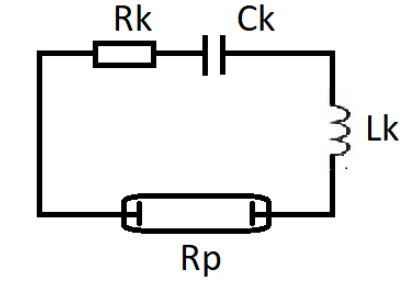
\includegraphics[width=8cm]{sch}}
\caption{Схема разрядного контура.}
\label{fig:image}
\end{figure}

Начальные условия: $t = 0, I = I_0, U = U_0$.

Здесь $I, U$ -- ток и напряжение на конденсаторе.

Сопротивление $R_p$ рассчитать по формуле $R_p = \frac{I_p}{2 \pi R^2 \int\limits_0^1 \sigma(T(z))zdz}$

Для функции $T(z)$ применить выражение $T(z) = T_0 + (T_w - T_0)z^m$.

Параметры $T_0, m$ находятся интерполяцией из табл.1 при известном токе $I$.
Коэффициент электропроводности $\sigma(T)$ зависит от $T$ и рассчитывается интерполяцией из  табл.2.

Параметры разрядного контура:

$R = 0.35$ см

$L_e = 12$ см

$L_k = 187 \cdot 10 ^{-6}$ Гн

$C_k = 268 \cdot 10^{-6}$ Ф

$R_k = 0.25$ Ом

$U_{co} = 1400$ В

$I_0 = 0..3$ А

$T_w = 2000$ К

\begin{table}
\caption{\label{tab:canonsummary} $I, T_0, m$}
\begin{center}
\begin{tabular}{|c|c|c|}
\hline
$I$, А & $T_0$, К & m \\
\hline
0.5 & 6730 & 0.50 \\
1 & 6790 & 0.55 \\
5 & 7150 & 1.7 \\
10 & 7270 & 3 \\
50 & 8010 & 11 \\
200 & 9185 & 32 \\
400 & 10010 & 40 \\
800 & 11140 & 41 \\
1200 & 12010 & 39 \\
\hline
\end{tabular}
\end{center}
\end{table} 

\begin{table}
\caption{\label{tab:canonsummary} $T, \sigma $}
\begin{center}
\begin{tabular}{|c|c|}
\hline
$T$, К & $T_0$, 1/Ом см \\
\hline
4000 & 0.031 \\
5000 & 0.27 \\
6000 & 2.05 \\
7000 & 6.06 \\
8000 & 12.0 \\
9000 & 19.9 \\ 
10000 & 29.6 \\
11000 & 41.1 \\
12000 & 54.1 \\
13000 & 67.7 \\
14000 & 81.5 \\
\hline
\end{tabular}
\end{center}
\end{table} 

\subsection*{Задание}

Необходимо построить следующие графики.

\begin{enumerate}
	\item Графики зависимости  от времени импульса $T$ : $I(t), U(t), R_p(t), I(t) \cdot R_p(t), T_0(t)$ при заданных выше параметрах. На одном из графиков привести результаты вычислений двумя методов разных порядков точности. Показать, как влияет выбор метода на шаг сетки.
	\item График зависимости $I(t) $ при $R_k + R_p = 0$. Обратить внимание на то, что в этом случае колебания тока будут не затухающими.
	\item График зависимости $I(t) $при $R_k = 200$ Ом в интервале  значений $t$ 0-20 мкс.
\end{enumerate}

\subsection*{Необходимые теоретические сведения}
\subsubsection*{Метод Рунге-Кутта второго порядка точности}

Имеем систему уравнений вида
\begin{equation*}
 \begin{cases}
   u'(x) = f(x, u(x)) \\
   u(\xi) = \eta
 \end{cases}
\end{equation*}

Получим формулы второго порядка точности метода Рунге-Кутта.

$u'_n = f(x_n, u_n)$

$y_{n+1} = y_n + h_n [(1 - \alpha) f(x_n, y_n) + \alpha f(x_n + \frac{h_n}{2 \alpha}, y_n + \frac{h_n}{2 \alpha}f(x_n, y_n))]$

Обычно $\alpha = 1$ или 0.5.

При $\alpha = 0.5$ получаетя неявный метод трапеций, а при $\alpha = 1$ -- метод средних. 

\subsubsection*{Метод Рунге-Кутта четвертого порядка точности}

Имеем систему уравнений вида
\begin{equation*}
 \begin{cases}
   u'(x) = f(x, u(x)) \\
   u(\xi) = \eta
 \end{cases}
\end{equation*}

Тогда

$y_{n+1} = y_n + \frac{k_1 + 2k_2 + 2k_3 + k_4}{6}$

$k_1 = h_n f(x_n, y_n)$

$k_2 = h_n f(x_n + \frac{h_n}{2}, y_n + \frac{k_1}{2})$

$k_3 = h_n f(x_n + \frac{h_n}{2}, y_n + \frac{k_2}{2})$

$k_4 = h_n f(x_n + h_n, y_n + k_3)$

Рассмотрим обобщение формулы на случай двух переменных. Пусть дана система

\begin{equation*}
 \begin{cases}
   u'(x) = f(x, u, v) \\
   v'(x) = \varphi(x, u, v) \\
   v(\xi) = v_0 \\
   u(\xi) = u_0 \\
 \end{cases}
\end{equation*}

Тогда

$y_{n+1} = y_n + \frac{k_1 + 2k_2 + 2k_3 + k_4}{6}$

$z_{n+1} = z_n + \frac{q_1 + 2q_2 + 2q_3 + q_4}{6}$

$k_1 = h_n f(x_n, y_n, z_n)$

$k_2 = h_n f(x_n + \frac{h_n}{2}, y_n + \frac{k_1}{2}, z_n + \frac{q_1}{2})$

$k_3 = h_n f(x_n + \frac{h_n}{2}, y_n + \frac{k_2}{2}, z_n + \frac{q_2}{2})$

$k_4 = h_n f(x_n + h_n, y_n + k_3, z_n + q_3)$

$q_1 = h_n \varphi(x_n, y_n, z_n)$

$q_2 = h_n \varphi(x_n + \frac{h_n}{2}, y_n + \frac{k_1}{2}, z_n + \frac{q_1}{2})$

$q_3 = h_n \varphi(x_n + \frac{h_n}{2}, y_n + \frac{k_2}{2}, z_n + \frac{q_2}{2})$

$q_4 = h_n \varphi(x_n + h_n, y_n + k_3, z_n + q_3)$

\subsection*{Код программы}

\begin{lstlisting}[label=code1,caption=\text{Класс MyApp.}]
import sys
from PyQt5 import QtWidgets
from PyQt5.QtWidgets import QMessageBox

from Modeller import Modeller
from Ui_mainwindow import Ui_MainWindow

class MyApp(QtWidgets.QMainWindow):
    def __init__(self):
        super(MyApp, self).__init__()
        self.ui = Ui_MainWindow()
        self.ui.setupUi(self)

        self.ui.run_button.clicked.connect(self.run)
        self.ui.set_default_btn.clicked.connect(self.set_defaults)

        self.defaults = {"R"      : 0.35,
                         "Le"     : 12,
                         "Lk"     : 187e-6,
                         "Ck"     : 268e-6,
                         "Rk"     : 0.25,
                         "Uc0"    : 1400,
                         "I0"     : 0.5,
                         "Tw"     : 2000,
                         "Tstart" : 0,
                         "Tend"   : 0.0006,
                         "Tstep"  : 1e-6}
        self.set_defaults()
        self.data = {}

    def set_defaults(self):
        self.ui.lineEdit_r.setText(str(self.defaults.get("R")))
        self.ui.lineEdit_le.setText(str(self.defaults.get("Le")))
        self.ui.lineEdit_lk.setText(str(self.defaults.get("Lk")))
        self.ui.lineEdit_ck.setText(str(self.defaults.get("Ck")))
        self.ui.lineEdit_rk.setText(str(self.defaults.get("Rk")))
        self.ui.lineEdit_uc0.setText(str(self.defaults.get("Uc0")))
        self.ui.lineEdit_i0.setText(str(self.defaults.get("I0")))
        self.ui.lineEdit_tw.setText(str(self.defaults.get("Tw")))
        self.ui.lineEdit_tstart.setText(str(self.defaults.get("Tstart")))
        self.ui.lineEdit_tend.setText(str(self.defaults.get("Tend")))
        self.ui.lineEdit_tstep.setText(str(self.defaults.get("Tstep")))

    def run(self):
        if self.check():
            mdlr = Modeller(self.data)
            isequal = self.ui.checkBox.isChecked()
            mdlr.compute(isequal)
        else:
            self.msg_box("Error!", "Error! Incorrect input!", QMessageBox.Critical)
    
    def msg_box(self, title, message, type):
        msg = QMessageBox(self)
        msg.setIcon(type)
        msg.setWindowTitle(title)
        msg.setText(message)
        msg.addButton('Ok', QMessageBox.AcceptRole)
        msg.exec()

    def check(self):
        try:
            self.data["R"] = float(self.ui.lineEdit_r.text())
            self.data["Le"] = float(self.ui.lineEdit_le.text())
            self.data["Lk"] = float(self.ui.lineEdit_lk.text())
            self.data["Ck"] = float(self.ui.lineEdit_ck.text())
            self.data["Rk"] = float(self.ui.lineEdit_rk.text())
            self.data["Uc0"] = float(self.ui.lineEdit_uc0.text())
            self.data["I0"] = float(self.ui.lineEdit_i0.text())
            self.data["Tw"] = float(self.ui.lineEdit_tw.text())
            self.data["Tstart"] = float(self.ui.lineEdit_tstart.text())
            self.data["Tend"] = float(self.ui.lineEdit_tend.text())
            self.data["Tstep"] = float(self.ui.lineEdit_tstep.text())
        except ValueError:
            return False
        return True


def main():
    app = QtWidgets.QApplication(sys.argv)
    window = MyApp()
    window.show()
    app.exec_()


if __name__ == '__main__':
    main()


\end{lstlisting}

\begin{lstlisting}[label=code1,caption=\text{Класс Modeller.}]
from math import pi
from scipy.interpolate import InterpolatedUnivariateSpline, CubicSpline
from matplotlib import pyplot as plt
from numpy import arange
from scipy import integrate

class Modeller():
    def __init__(self, data):
        self.data = data

        self.itk = [[0.5, 6700, 0.5],
                    [1,	6790, 0.55],
                    [5,	7150, 1.7],
                    [10, 7270, 3],
                    [50, 8010, 11],
                    [200, 9185, 32],
                    [400, 10010, 40],
                    [800, 11140, 41],
                    [1200, 12010, 39]]
        
        self.tsigma = [
            [4000, 0.031],
            [5000, 0.27],
            [6000, 2.05],
            [7000, 6.06],
            [8000, 12.0],
            [9000, 19.9],
            [10000, 29.6],
            [11000, 41.1],
            [12000, 54.1],
            [13000, 67.7],
            [14000, 81.5]]

        self.m = None
        self.T0 = None
        #self.m4 = None
        #self.T04 = None
        self.simpsonN = 41

    def compute(self, isequal):
        tstart = self.data.get("Tstart")
        tend = self.data.get("Tend")
        tstep = self.data.get("Tstep")
        I0 = self.data.get("I0")
        Uc0 = self.data.get("Uc0")
        I04 = self.data.get("I0")
        Uc04 = self.data.get("Uc0")

        t_plot = []
        rp_plot = []
        rp_plot4 = []
        I_plot = []
        I_plot4 = []
        U_plot = []
        U_plot4 = []
        T0_plot = []
        IRp_plot = []
        IRp_plot4 = []

        for t in arange(tstart, tend, tstep):
            Rp = self.Rp(I0)
            if isequal:
                self.data['Rk'] = -Rp
            I0, Uc0 = self.runge_kutta2(I0, Uc0, tstep, Rp)

            t_plot.append(t)
            rp_plot.append(Rp)
            I_plot.append(I0)
            U_plot.append(Uc0)
            T0_plot.append(self.T0)
            IRp_plot.append(I0 * Rp)

            Rp4 = self.Rp(I04)
            if isequal:
                self.data['Rk'] = -Rp4
            I04, Uc04 = self.runge_kutta4(I04, Uc04, tstep, Rp4)
            rp_plot4.append(Rp4)
            I_plot4.append(I04)
            U_plot4.append(Uc04)
            IRp_plot4.append(I04 * Rp4)

        
        plt.figure(1)

        plt.suptitle("Методы Рунге-Кутта 2-го и 4-го порядка")
        plt.subplot(321)
        plt.plot(t_plot, rp_plot, label = '2-й порядок')
        plt.plot(t_plot, rp_plot4, label = '4-й порядок')
        plt.xlabel('t, с')
        plt.ylabel('Rp, Ом')
        plt.grid(True)
        plt.legend()

        plt.subplot(322)
        plt.plot(t_plot, I_plot, label = '2-й порядок')
        plt.plot(t_plot, I_plot4, label = '4-й порядок')
        plt.xlabel('t, с')
        plt.ylabel('I, А')
        plt.grid(True)
        plt.legend()

        plt.subplot(323)
        plt.plot(t_plot, U_plot, label = '2-й порядок')
        plt.plot(t_plot, U_plot4, label = '4-й порядок')
        plt.xlabel('t, с')
        plt.ylabel('U, В')
        plt.grid(True)
        plt.legend()

        plt.subplot(324)
        plt.plot(t_plot, T0_plot)
        plt.xlabel('t, с')
        plt.ylabel('T0, К')
        plt.grid(True)
        
        plt.subplot(325)
        plt.plot(t_plot, IRp_plot, label = '2-й порядок')
        plt.plot(t_plot, IRp_plot4, label = '4-й порядок')
        plt.xlabel('t, с')
        plt.ylabel('I * Rp, В')
        plt.grid(True)
        plt.legend()

        plt.show()

    def Rp(self, I):
        I_table = []
        itk_len = len(self.itk)
        for i in range(itk_len):
            I_table.append(self.itk[i][0])
        T0_table = []
        for i in range(itk_len):
            T0_table.append(self.itk[i][1])

        m_table = []
        for i in range(itk_len):
            m_table.append(self.itk[i][2])
        
        self.m = self.interpolate(I, I_table, m_table)
        self.T0 = self.interpolate(I, I_table, T0_table)

        intgl = self.simpson(self.integrand, 0, 1, self.simpsonN)
        #intgl = integrate.simps(self.integrand, 0, 1)
        #intgl = integrate.quad(self.integrand, 0, 1)
        Rp = self.data.get("Le") / (2 + pi * (self.data.get("R") ** 2) * intgl)
        return Rp

    def integrand(self, z):
        return self.sigma(self.Tz(z)) * z
        

    def Tz(self, z):
        return (self.T0 + (self.data.get("Tw") - self.T0) * (z ** self.m))
    
    def f(self, U, I, Rp):
        Rk = self.data.get("Rk")
        Lk = self.data.get("Lk")
        return ((U - (Rk + Rp) * I) / Lk)

    def phi(self, U, I):
        Ck = self.data.get("Ck")
        return - I / Ck
    
    def runge_kutta4(self, yn, zn, hn, Rp):
        hn2 = hn / 2

        k1 = hn * self.f(zn, yn, Rp)
        q1 = hn * self.phi(zn, yn)

        k2 = hn * self.f(zn + k1 / 2, yn + q1 / 2, Rp)
        q2 = hn * self.phi(zn + k1 / 2, yn + q1 / 2)
        
        k3 = hn * self.f(zn + k2 / 2, yn + q2 / 2, Rp)
        q3 = hn * self.phi(zn + k2 / 2, yn + q2 / 2)

        k4 = hn * self.f(zn + k3, yn + q3, Rp)
        q4 = hn * self.phi(zn + k3, yn + q3)

        y_next = yn + (k1 + 2 * k2 + 2 * k3 + k4) / 6
        z_next = zn + (q1 + 2 * q2 + 2 * q3 + q4) / 6

        return y_next, z_next




    def runge_kutta2(self, yn, zn, hn, Rp): # I, U
        alpha = 0.5

        nh = hn / (2 * alpha)
        k1 = self.f(zn, yn, Rp)
        q1 = self.phi(zn, yn)
        k2 = self.f(zn + nh * q1, yn + nh * k1, Rp)
        q2 = self.phi(zn + nh * q1, yn + nh * k1)
        next_y = yn + hn * ((1 - alpha) * k1 + alpha * k2)
        next_z = zn + hn * ((1 - alpha) * q1 + alpha * q2)
        return next_y, next_z

    def sigma(self, T):
        T_table = []
        len_tsigma = len(self.tsigma)
        for i in range(len_tsigma):
            T_table.append(self.tsigma[i][0])
        sigma_table = []
        for i in range(len_tsigma):
            sigma_table.append(self.tsigma[i][1])
        
        return self.interpolate(T, T_table, sigma_table)
    
    def interpolate(self, I_known, kn_col1, kn_col2):
        #res = InterpolatedUnivariateSpline(kn_col1, kn_col2, k = 1)
        res = CubicSpline(kn_col1, kn_col2, extrapolate=True)
        return float(res(I_known))
    
    def simpson(self, func, a, b, N):
        h = float((b - a) / N)
        res_sum = 0
        for step in range(N):
            x1 = a + step * h
            x2 = a + (step + 1) * h
            res_sum += (x2 - x1) / 6.0 *(func(x1) + 4.0 * func(0.5 * (x1 + x2)) + func(x2))
        return res_sum

\end{lstlisting}

\subsection*{Результаты работы программы}

На рисунке 2 представлен графический интерфейс программы.

На рисунке 3 представлены результаты работы программы для методов Рунге-Кутта второго (синий) и четвертого (оранжевый) порядков точности для заданных по умолчанию параметров.

На рисунках 4-6 представлены результаты работы прогрммы с разным шагом. Из рисунков видно, что при уменьшении шага результаты методов 2-го и 4-го порядка совпадают, а при увеличении шага разница меджду результатами двух методов увеличивается. 

На рисунке 7 представлен график зависимости $I(t) $ при $R_k + R_p = 0$. При отсутствии сопротивления контур превращается в колебательный, поэтому колебания незатухающие.

На рисунке 8 представлен график зависимости $I(t) $при $R_k = 200$ Ом в интервале  значений $t$ 0-20 мкс.


\newpage

\begin{figure}[!h]
\center{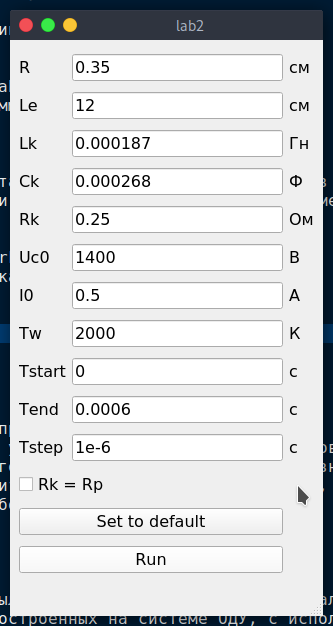
\includegraphics[width=8cm]{interf}}
\caption{Графический интерфейс программы.}
\label{fig:image}
\end{figure}

\newpage

\begin{figure}[!h]
\center{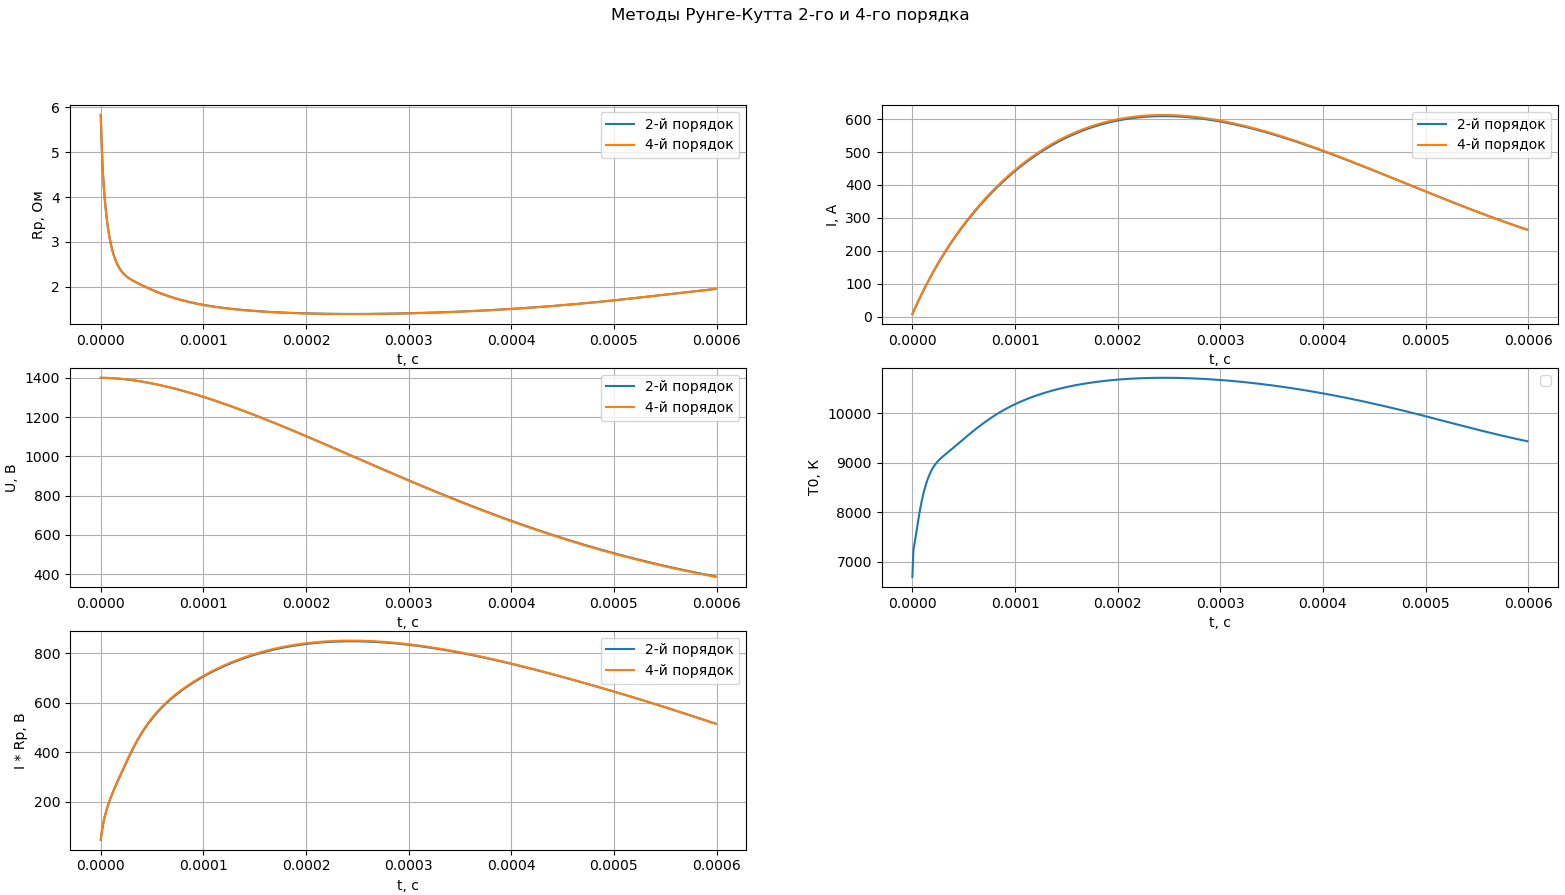
\includegraphics[width=17cm]{def}}
\caption{Шаг 1e-6.}
\label{fig:image}
\end{figure}

\begin{figure}[!h]
\center{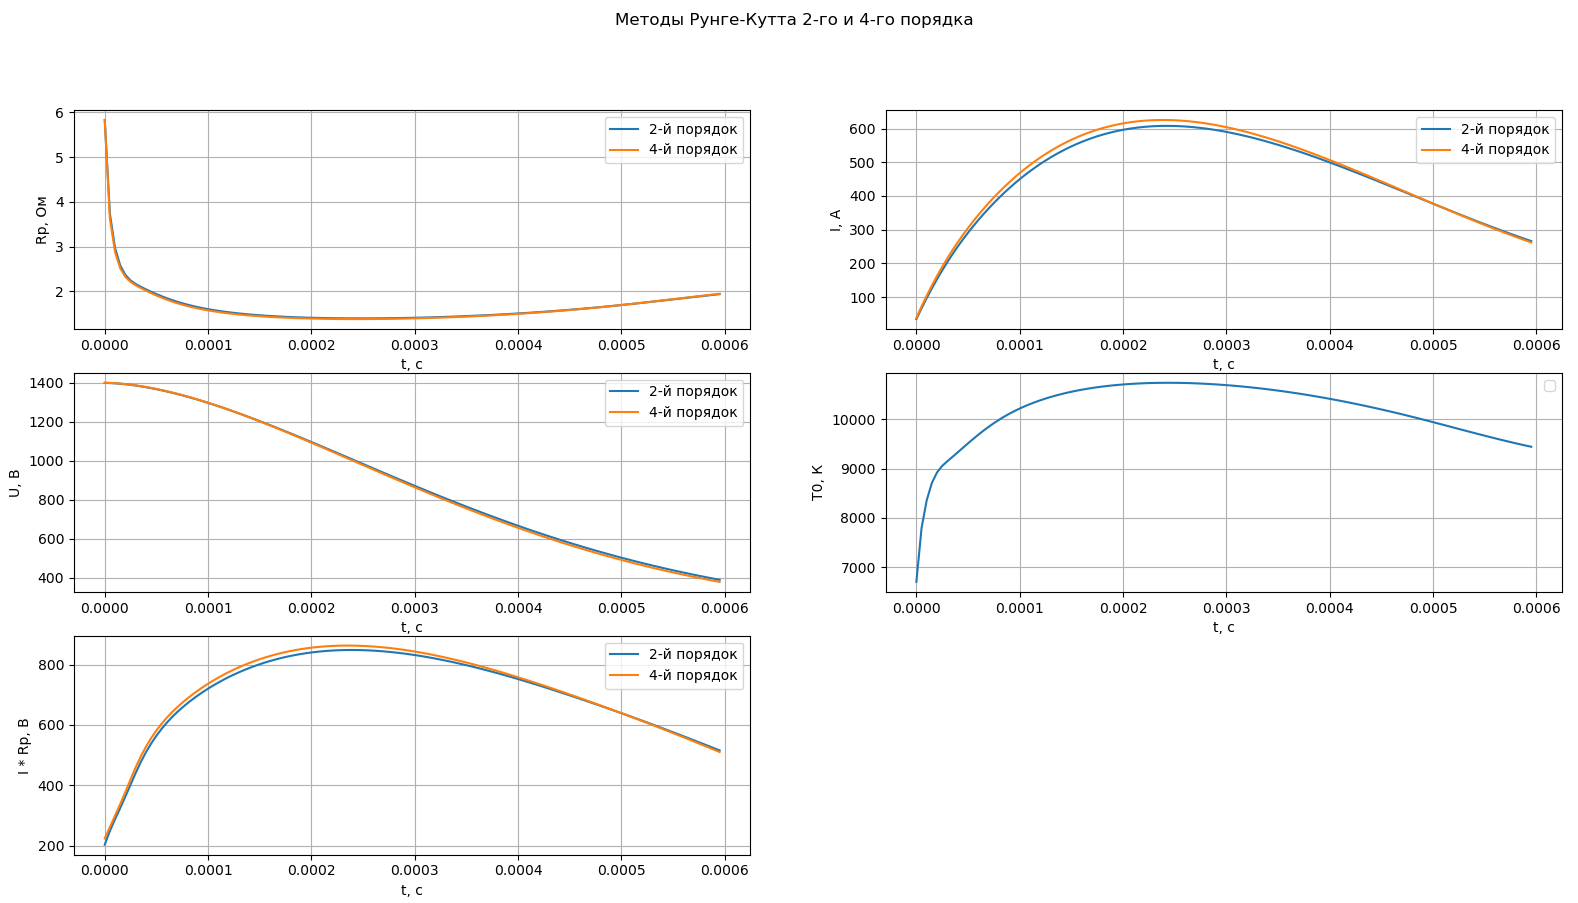
\includegraphics[width=17cm]{5e-6}}
\caption{Шаг 5e-6.}
\label{fig:image}
\end{figure}

\newpage

\begin{figure}[!h]
\center{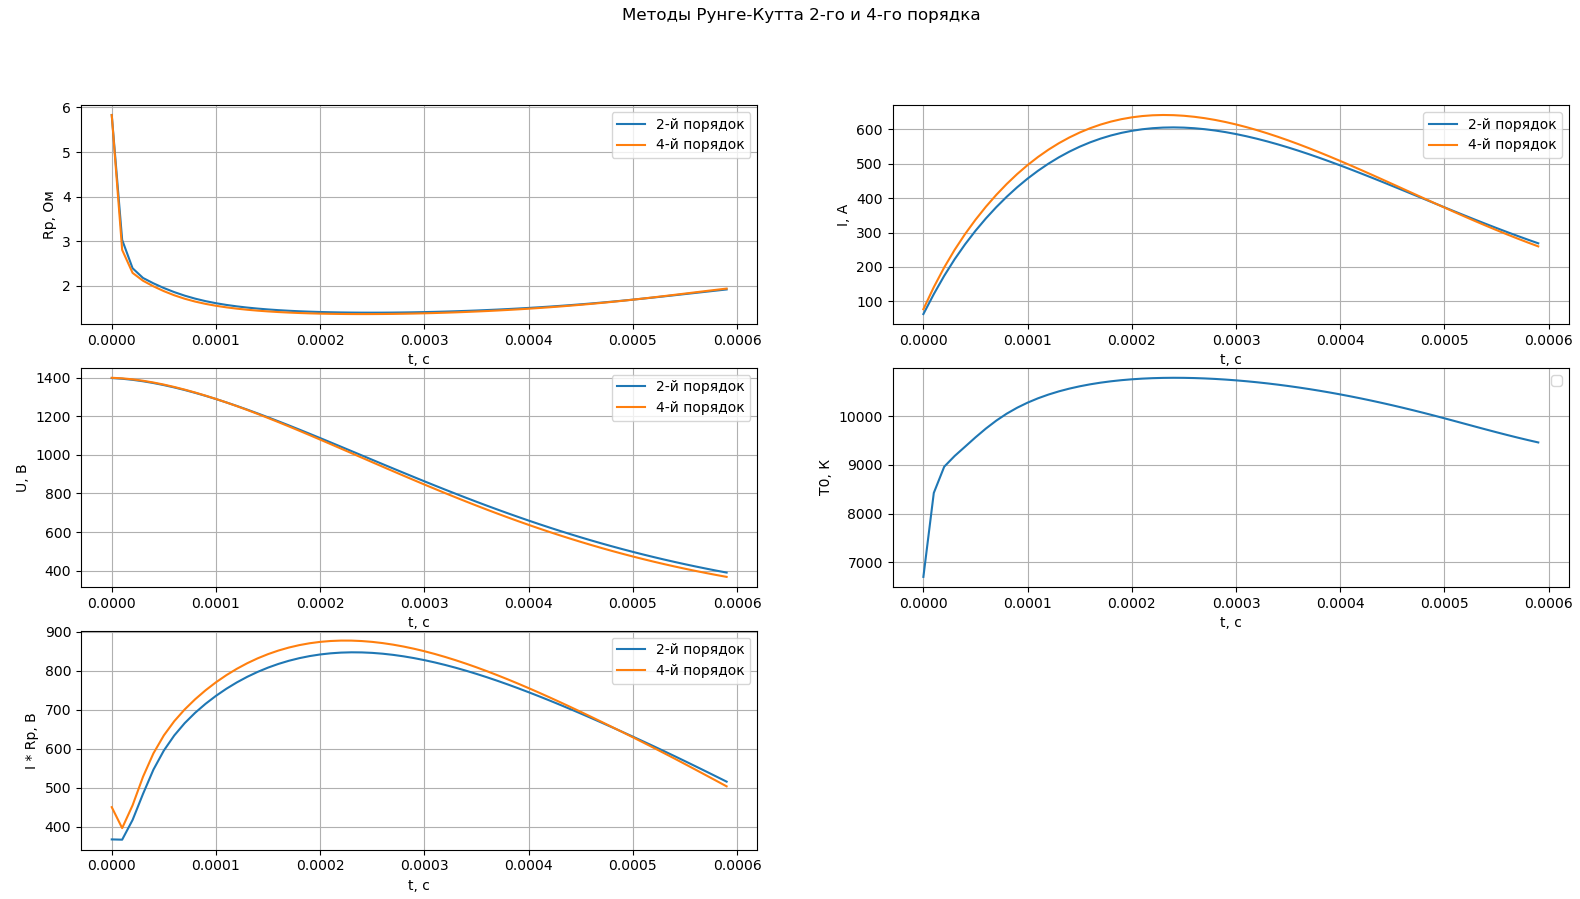
\includegraphics[width=17cm]{1e-5}}
\caption{Шаг 1e-5.}
\label{fig:image}
\end{figure}

\begin{figure}[!h]
\center{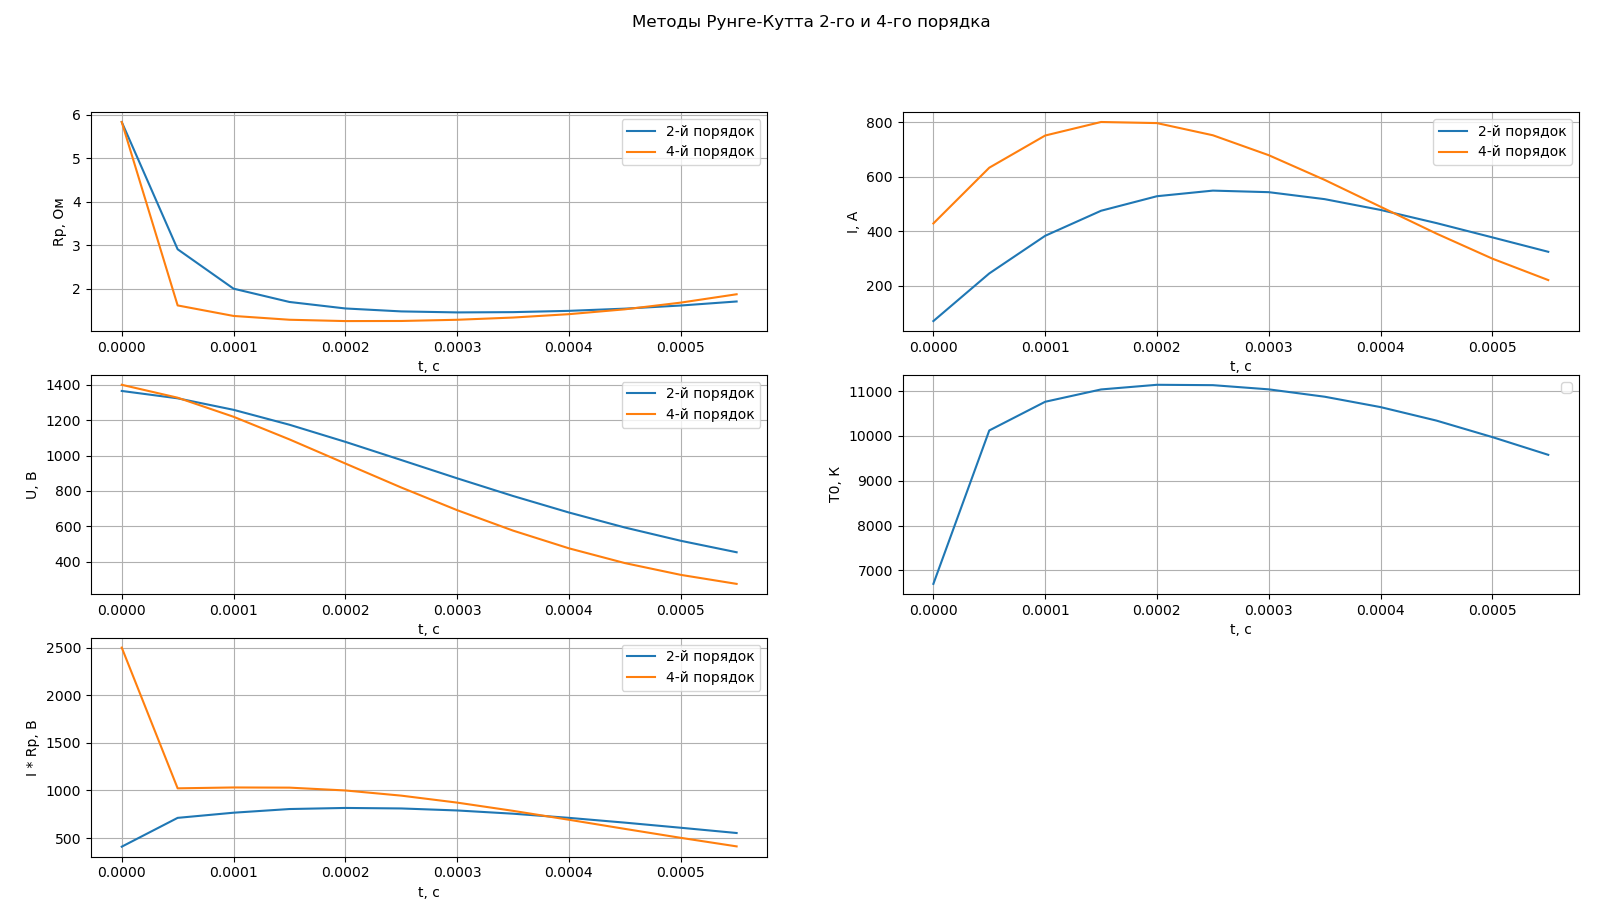
\includegraphics[width=17cm]{5e-5}}
\caption{Шаг 5e-5.}
\label{fig:image}
\end{figure}

\begin{figure}[!h]
\center{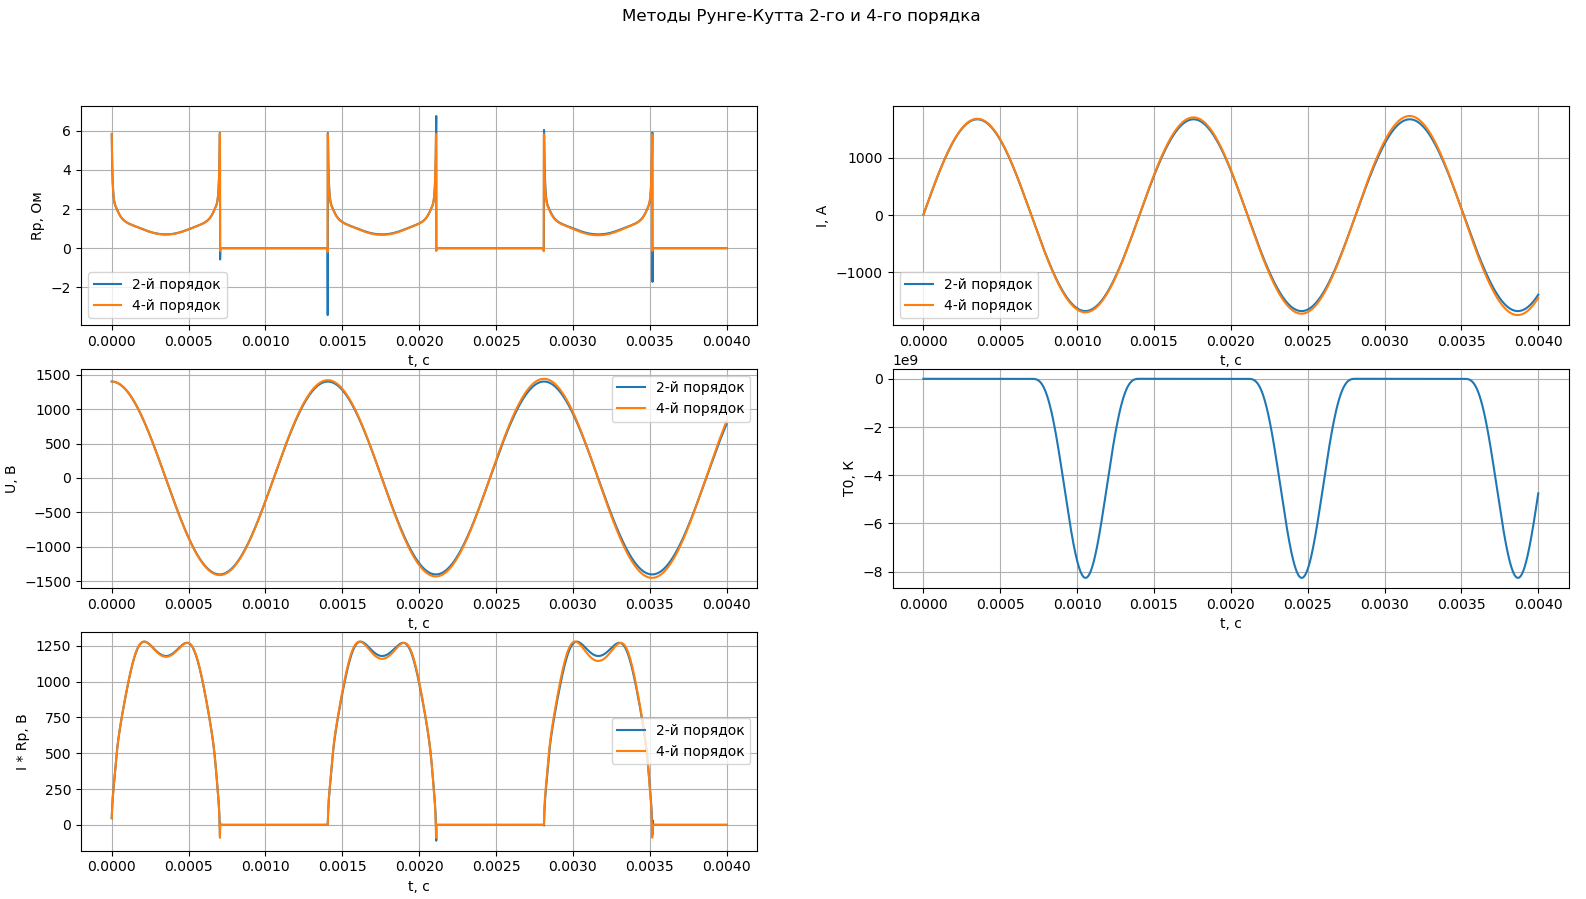
\includegraphics[width=17cm]{kol}}
\caption{Незатухающие колебания.}
\label{fig:image}
\end{figure}

\begin{figure}[!h]
\center{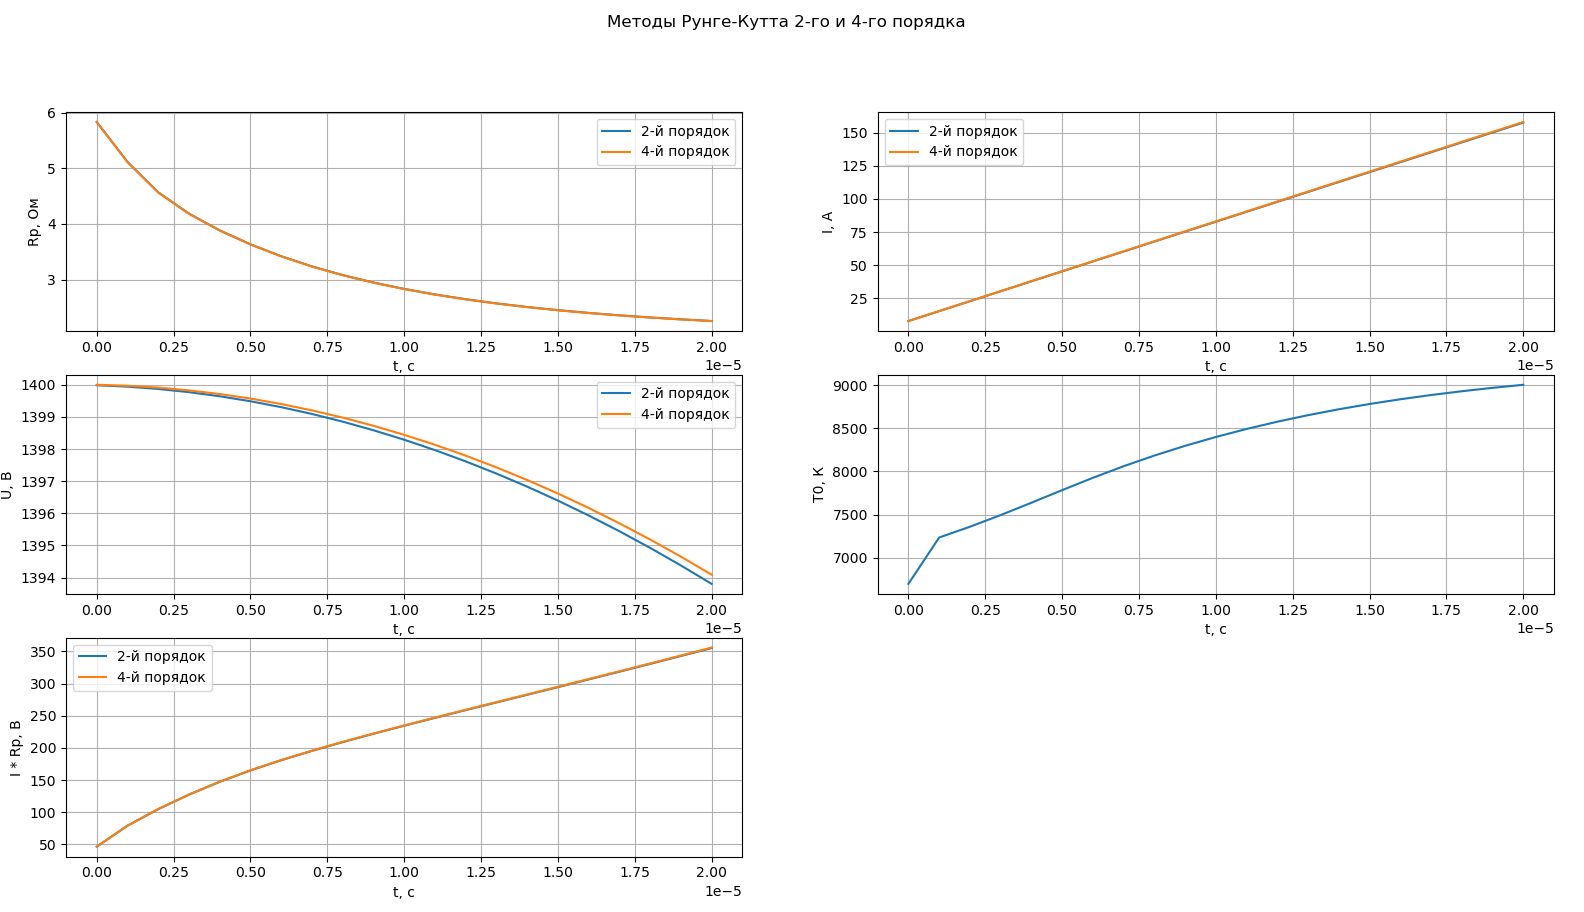
\includegraphics[width=17cm]{om200}}
\caption{$R_k = 200$ Ом.}
\label{fig:image}
\end{figure}

\newpage
\subsection*{Ответы на вопросы}

\begin{enumerate}
	\item Какие способы тестирования программы можно предложить?
	
	Правильность работы программы можно определить по виду графиков. Например,
можно проверить, что программа правильно ведет себя при вводе большого значения
сопротивления или в случае, когда сумма сопротивлений контура равна нулю (контур
обращается в колебательный, колебания не затухают).

	Тестирование программы также необходимо проводить при различных значениях шага. При достижении некоторого значения шага его дальнейшее уменьшение не повлияет на результат (на вид графиков). Это означает, что найден точный результат. Однако стоит учитывать, что слишком маленький шаг может привести к погрешности округления.
	
	Кроме этого, можно сравнивать результаты работы двух методов: при маленьком шаге их результаты должны совпадать.
	
	\item Получите систему разностных уравнений для решения сформулированной задачи неявным методом трапеций. Опишите  алгоритм реализации полученных уравнений.

Метод трапеций:

\begin{equation*}
 u_{n+1} = u_n + \int\limits_{x_n}^{x_{n+1}}f(x, u(x))dx 
\end{equation*}

\begin{equation*}
 y_{n+1} = y_n + \frac{h}{2}[f(x_n, y_n) + f(x_{n+1}, y_{n+1})] + O(h^2)
\end{equation*}

В нашей задаче имеем:

\begin{equation*}
 \begin{cases}
   \frac{dI}{dT} = \frac{Uc - (R_k + R_p(I))I}{L_k} = f(I, Uc)\\
   \frac{dU}{dT} = -\frac{I}{C_k} = g(I)
 \end{cases}
\end{equation*}


$ I_{n+1} = I_n + \frac{h}{2}[f(I_n, Uc_n) + f(I_{n+1}, Uc_{n+1})]$ 
 
$ Uc_{n+1} = Uc_n + \frac{h}{2}[g(I_n) + g(I_{n+1})] $

~\

$ I_{n+1} = I_n + \frac{h}{2}[f(I_n, Uc_n) + f(I_{n+1}, Uc_{n+1})] $

$ Uc_{n+1} = Uc_n + \frac{h}{2}[g(I_n) + g(I_{n+1})] $

~\

$ I_{n+1} = I_n + \frac{h}{2}[\frac{Uc_n - (R_k + R_p(I_n))I_n + Uc_{n+1} - (R_k + R_p(I_{n+1}))I_{n+1}}{L_k}]$

$ Uc_{n+1} = Uc_n - \frac{h}{2}[\frac{I_n + I_{n+1}}{C_k}] $

Отсюда можно выразить $I_{n+1}$:

$I_{n+1} = \frac{C_k \cdot I_n + C_k \cdot h \cdot Uc_n - C_k \cdot h \cdot I_n(R_k + R_p(I_n)) + h \cdot Uc_n \cdot C_k - h^2 \cdot I_n}{2 \cdot C_k \cdot L_k + h^2 + C_k \cdot h (R_k + R_p(I_{n+1}))}$

Это уравнение можно решить методом простой итерации. После нахождения $I_{n+1}$ находим $Uc_{n+1}$.

	\item Из каких соображений проводится выбор того или иного метода, учитывая, что чем выше порядок точности метода, тем он более сложен?
	
	На выбор того или иного метода влияет два фактора: требуемая точность результата и время, за которое необходимо получить результат. Более точные методы, как правило, требуют больше времени, а менее точные -- меньше времени. 
	
	Рассмотрим погрешность метода Рунге-Кутта второго порядка при $\alpha = 1$:
	
	$R = \frac{X_N - X_0}{24} \cdot h^2 \cdot \max_{\{x_0 \leq x \leq x_n\}} |f''(x)|$
	
	Рассмотрим погрешность метода Рунге-Кутта четвертого порядка:
	
	\newcounter{ff}
	\setcounter{ff}{4}
	$R = \frac{X_N - X_0}{2880} \cdot h^4 \cdot \max_{\{x_0 \leq x \leq x_n\}} |f^{\Roman{ff}}(x)|$
    
    Таким образом, при выборе метода необходимо учитывать абсолютное значение производной (второй в случае метода второго порядка и четвертой в случае метода четвертого порядка).
    Может возникнуть такая ситуация, когда из-за значения производной метод второго порядка будет давать более точный результат и при этом его сложность будет ниже.
\end{enumerate}

\subsection*{Вывод}

Таким образом, в ходе данной работы были получены навыки разработки  алгоритмов решения задачи Коши при реализации моделей, построенных на системе ОДУ, с использованием методов Рунге-Кутта 2-го и 4-го порядков точности.


\end{document}

\end{document}